\subsubsection{\gls{pcb} Hardware Elements}

The hardware subsystem forms the foundation of the drone, integrating all power, control, and sensing elements on a custom \gls{pcb}. It is designed to be compact, lightweight, and serviceable while maintaining electrical reliability, \gls{emi} resilience, and thermal performance. Fig.~\ref{fig:pcb-sections} and Fig.~\ref{fig:pcb-final} illustrates the overall hardware design. The prototype \gls{pcb} iterations are given in Appendix~\ref{app:pcb-prototypes}. 

The intent and the description of various hardware elements is given Table~\ref{tab:hardware-elements}.

\begin{figure}[H]
    \centering
    \captionsetup{justification=centering, margin=1cm}
    \begin{subfigure}[b]{0.48\textwidth}
        \centering
        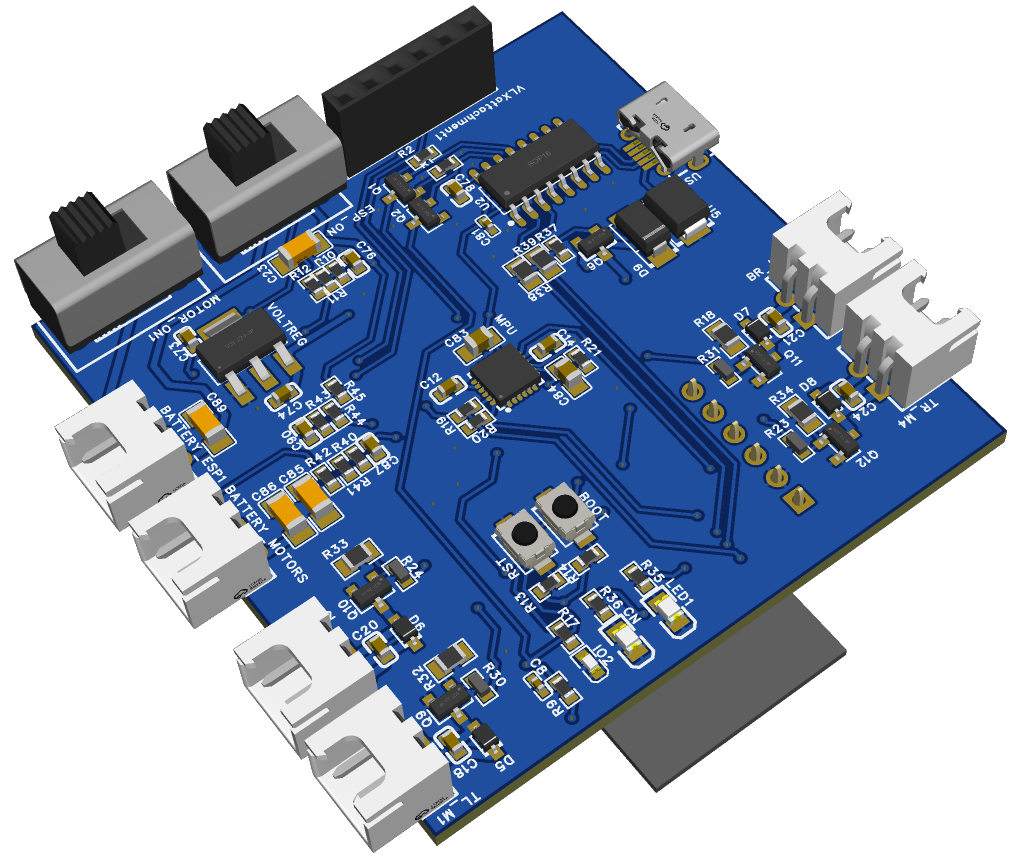
\includegraphics[width=\textwidth]{img/final-pcb2.png}
        \caption{Front}
        \label{fig:pcb-front}
    \end{subfigure}
    \hfill
    \begin{subfigure}[b]{0.48\textwidth}
        \centering
        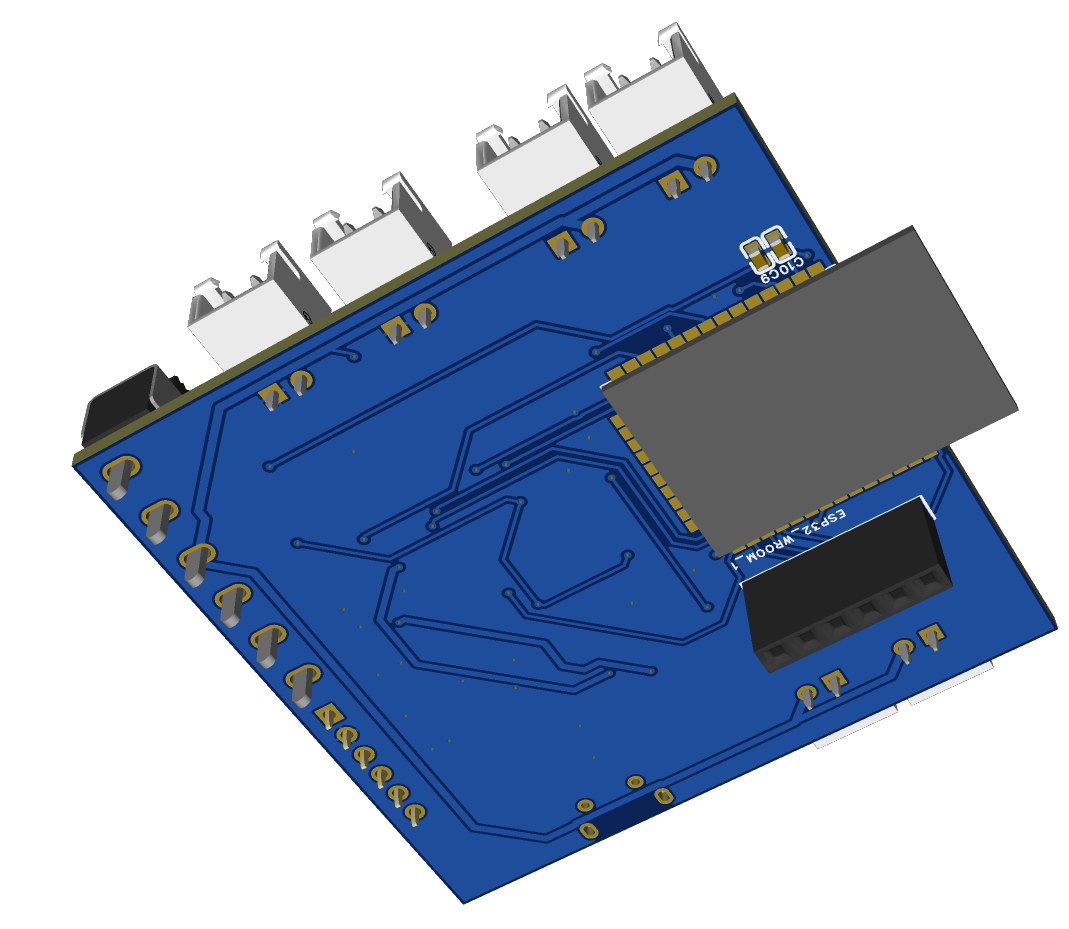
\includegraphics[width=\textwidth]{img/final-pcb-back.png}
        \caption{Back}
        \label{fig:pcb-back}
    \end{subfigure}
    \caption{Front and back sides of the final PCB design.}
    \label{fig:pcb-final}
\end{figure}

\begin{figure}[H]
    \centering
    \captionsetup{justification=centering, margin=1cm}
    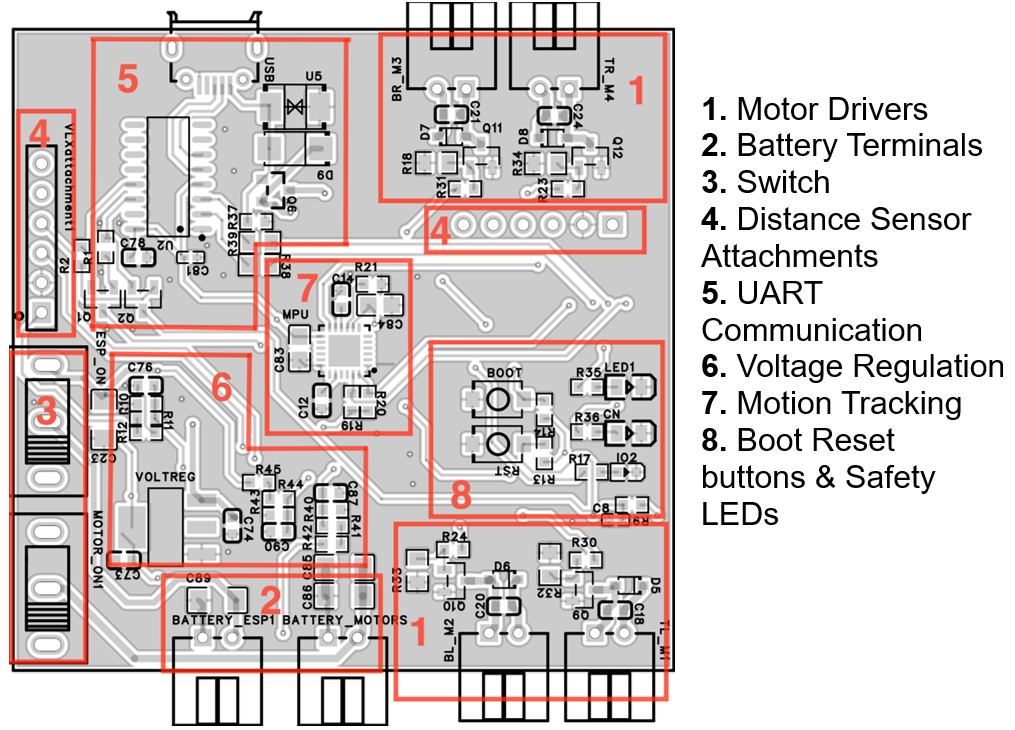
\includegraphics[width=0.6\textwidth]{img/pcb-sections3.PNG}
    \caption{Areas of \gls{pcb} design}
    \label{fig:pcb-sections}
\end{figure}

\begin{longtable}{@{}p{2cm} p{6.9cm} p{6.9cm}@{}}
\caption{Summary of Hardware Elements and Their Design Intent}
\label{tab:hardware-elements} \\
\toprule
\textbf{Element} & \textbf{Intent \& Requirements} & \textbf{Design Description} \\ 
\midrule
\textbf{Motor Drivers} &
\textit{Intent:} Drive brushed motors safely with low \gls{emi} and adequate thermal margin. \newline
\textit{Requirements:} R.23 low cost; A.R.6 case temperature $\leq 85~^{\circ}$C; supply droop $\leq 10\%$ at full duty; \gls{emi} interference-free I\textsuperscript{2}C communication. &
Motor drivers are placed near \gls{pcb} edges to minimise path resistance and \gls{emi}. Flyback diodes and RC snubbers reduce transients; short, wide power returns and local decoupling capacitors enhance current stability. \\ 
\midrule
\textbf{Battery Terminals} &
\textit{Intent:} Provide a robust and safe connection for 1S/2S Li-ion/\gls{lipo} power. \newline
\textit{Requirements:} R.18/A.R.2 single-battery operation; reverse insertion blocked; voltage drop $\leq 100$~mV at max current. &
Locking \gls{jst}-style connector with keyed housing ensures polarity. Bulk capacitors stabilize voltage input; wide copper pours minimise resistance to \gls{ldo} and driver rails. \\ 
% \midrule
% \textbf{Power Switch (Enable)} &
% \textit{Intent:} Allow user-controlled power activation without arcing or brownout. \newline
% \textit{Requirements:} R.17 safety handling; voltage sag $\leq 5\%$ on 3.3~V rail. &
% \gls{rc} debounce implemented; switch positioned away from propellers with silkscreen labels and visual LED indicators for power status. \\ 
\midrule
\textbf{Distance Sensor Attachments} &
\textit{Intent:} Enable obstacle avoidance and altitude hold. \newline
\textit{Requirements:} R.11/R.12 obstacle sensing; I\textsuperscript{2}C error rate = 0 during PWM activity. &
Two 4-pin headers (GND/VCC/SCL/SDA) with onboard pull-ups for optional sensor modules; mechanical mounting aligns with forward and downward sensing directions. \\ 
\midrule
\textbf{UART/USB Communication} &
\textit{Intent:} Support flashing and telemetry without disassembly. \newline
\textit{Requirements:} AF.R.9 flashing success $\geq 99\%$; A.R.10 accessible during assembly; \gls{esd} robustness. &
CP2102/CH340 bridge with \gls{esd} protection and reverse-current Schottky diode on 5~V. Connector side-mounted for tool-free firmware updates. \\ 
\midrule
\textbf{Voltage Regulation (3.3~V Rail)} &
\textit{Intent:} Provide stable, low-noise 3.3~V power for \gls{mcu} and \gls{imu}. \newline
\textit{Requirements:} Output within $\pm5\%$; regulator temp $\leq 85~^{\circ}$C under full load. &
Linear \gls{ldo} provides noise-free supply; distributed decoupling and thermal copper pours dissipate heat efficiently. \\ 
\midrule
\textbf{Motion Tracking (IMU)} &
\textit{Intent:} Deliver accurate attitude measurement with minimal vibration coupling. \newline
\textit{Requirements:} R.20 stabilisation; placement within $\pm3$~mm of centroid; reliable \gls{i2c}/\gls{spi} interface. &
\gls{imu} placed centrally for balanced dynamics; shielded traces and ground guards minimise noise; isolated from high-current return paths. \\ 
\midrule
\textbf{Power \& Control Interface} &
\textit{Intent:} Enable safe power control, system reset, and visual feedback during operation. \newline
\textit{Requirements:} R.17 safety handling; A.R.7/A.R.10 indicators visible at 0.5~m; voltage sag $\leq 5\%$ on 3.3~V rail; accessible with props installed. &
\gls{rc} debounce circuit ensures reliable power switching without arcing or brownout. BOOT/EN buttons are placed near the board edge for easy reach, with tri-state \glspl{led} indicating idle, active, and low-battery states. Clear silkscreen labels and spacing minimise user error and \gls{rf} interference. \\
\end{longtable}

%-------------------------------------------------------------%
\subsubsection{Frame Design Elements}

The frame provides mechanical protection, airflow, and structural support while accommodating sensors, cameras, and cabling. Each component was designed for serviceability, modularity, and weight efficiency while preserving the drone’s balance and stability.

\begin{figure}[H]
    \centering
    \captionsetup{justification=centering, margin=1cm}
    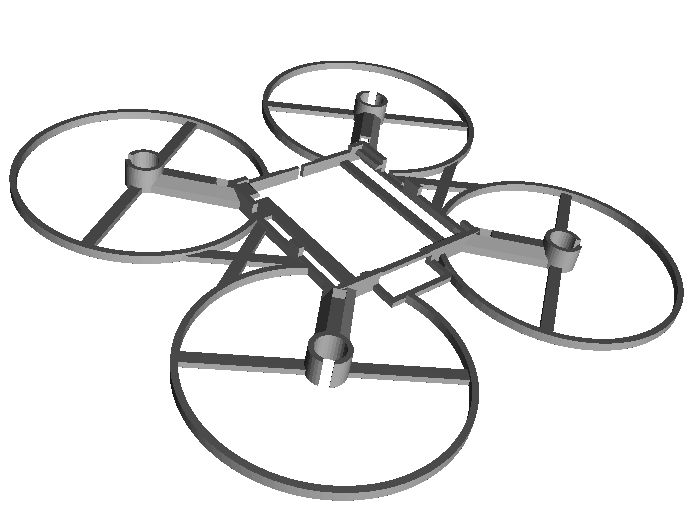
\includegraphics[width=0.5\textwidth]{img/main-frame.PNG}
    \caption{Frame design}
    \label{fig:frame}
\end{figure}

\begin{longtable}{@{}p{3.2cm} p{6.4cm} p{6.4cm}@{}}
\toprule
\textbf{Element} & \textbf{Intent \& Requirements} & \textbf{Design Description} \\ 
\midrule

\textbf{Camera Mount (Front Facing)} &
\textit{Intent:} Maintain clear \gls{fov} and low vibration for stable imaging. \newline
\textit{Requirements:} R.28/R.29 video; R.2/R.20 stability; quick-swap $\leq 60$~s. &
Snap-on carrier with compliant flexure arms isolates vibration; unobstructed optical path; easily replaceable. \\ 
\midrule

\textbf{Antenna \& LED Keep-Outs} &
\textit{Intent:} Ensure \gls{rf} integrity and \gls{led} visibility. \newline
\textit{Requirements:} A.R.7/A.R.10 indicators visible at 0.5~m; antenna free of obstruction. &
Keep-out zones near ESP32 antenna edge maintained; \glspl{led} exposed through open frame for visibility and heat dissipation. \\ 
\midrule

\textbf{Cable Management \& Strain Relief} &
\textit{Intent:} Prevent interference with propellers and ensure safe wiring. \newline
\textit{Requirements:} A.R.6 mechanical safety; cable retention $\geq$ 15~N. &
Dedicated tie-points and routing along arms; cables secured away from rotors and heat zones. \\ 
\midrule

\textbf{Serviceability \& Replacement} &
\textit{Intent:} Enable rapid repair and part replacement. \newline
\textit{Requirements:} Replaceable parts; print time $\leq$ 3~h for any component. &
Tool-less snap-fit assembly with modular arms and carriers; low-cost reprinting workflow. \\ 
\midrule

\textbf{Crash Protection \& Mass Control} &
\textit{Intent:} Absorb impact energy and protect electronics. \newline
\textit{Requirements:} R.23 cost/weight; prevent critical damage in collisions. &
Sacrificial \gls{petg} prop guards and legs designed to fail first, shielding \gls{pcb} and motors during impact. \\ 
\bottomrule
\end{longtable}